\section{Tutorial Hello World}
    Esta seção mostra os procedimentos realizados durante a leitura do tutorial \href{https://guides.github.com/activities/hello-world/}{\textit{"Hello World"}}.
    
    \subsection{Criando um repositório}
    Para realizar o tutorial, foi necessário utilizar minha conta no Github e criar um repositório. Escolhi o nome "Engenharia\_software\_1\_2020.1" pois armazenarei no repositório as atividades realizadas para a disciplina de Engenharia de Software 1.
    
    \begin{figure}[H]
        \caption{Repositório no Github}
        \vspace{0.5cm}
        \centering
        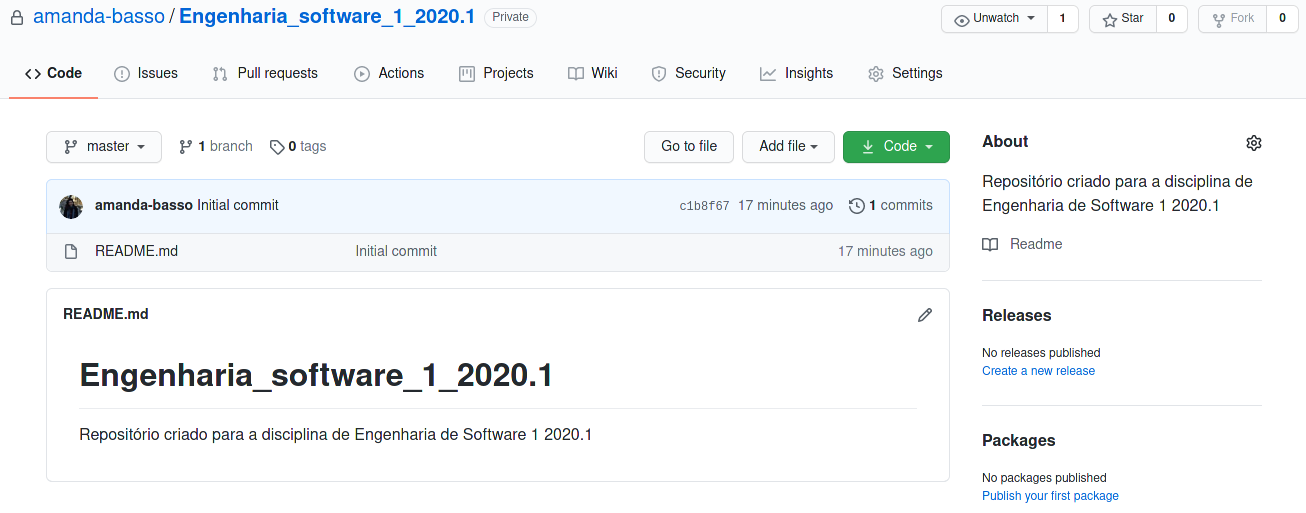
\includegraphics[width=15cm]{imagens/criacao_repositorio.png}
        \label{figura:repositorio_github}
    \end{figure}

    Embora tenha criado o repositório inicialmente como "privado", pretendo torná-lo público futuramente.
    \par Também vale ressaltar que foi iniciado com o arquivo \textit{README.md}, responsável por fornecer informações sobre o projeto armazenado no repositório. Também inseri, em seguida, o arquivo \textit{.gitignore}, que facilita o gerenciamento dos arquivos ao não rastrear arquivos que não desejo armazenar, como aqueles gerados ao compilar arquivos \textit{.tex}.
    
    \subsection{Criando um \textit{branch}}
    Criei um novo \textit{branch} chamado "tutoriais" onde, de fato, trabalhei adicionando arquivos, como o arquivo de formatação para o relatório.
    
    \begin{figure}[H]
        \caption{\textit{Branches} do projeto}
        \vspace{0.5cm}
        \centering
        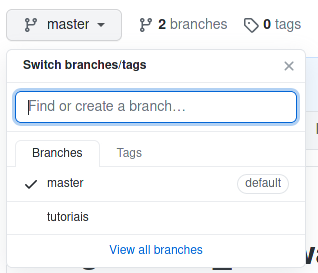
\includegraphics[width=5cm]{imagens/branch_tutoriais.png}
        \label{figura:branch_tutoriais}
    \end{figure}

    \subsection{Realizando modificações e \textit{commits}}
    Comecei a escrever os relatórios da disciplina e a armazená-los no \textit{branch} tutoriais. O resultado das modificações é exibido na imagem\ref{figura:changes}:
    
    \begin{figure}[H]
        \caption{Modificações no \textit{branch} tutoriais}
        \vspace{0.5cm}
        \centering
        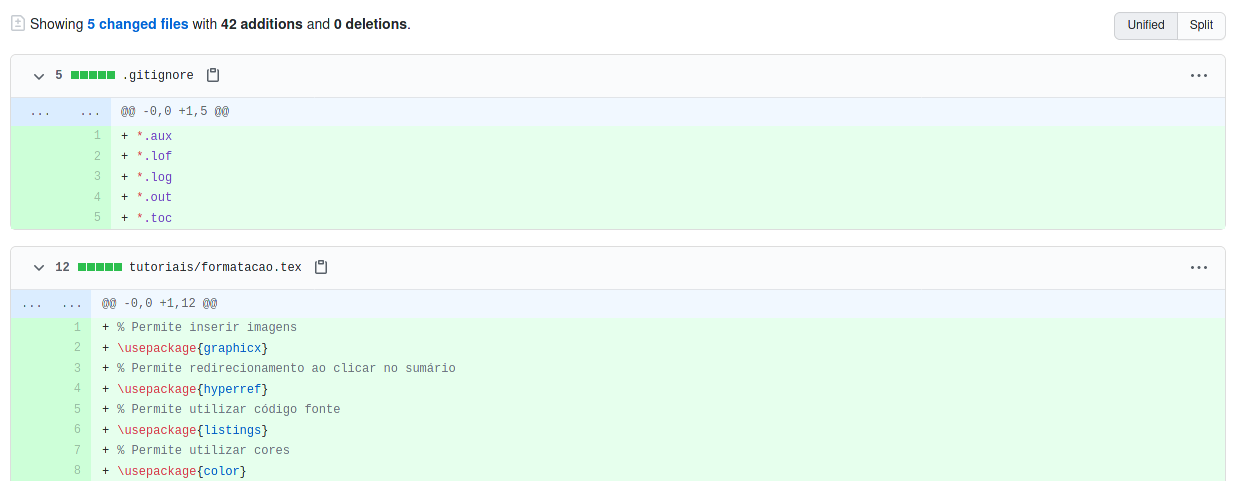
\includegraphics[width=15cm]{imagens/changes.png}
        \label{figura:changes}
    \end{figure}

    \subsection{Abrindo um \textit{Pull request}}
    Após realizar as modificações desejadas e salvá-las no \textit{branch} tutoriais, dei um \textit{pull request} para o \textit{branch master}. A imagem\ref{figura:comparing_changes} mostra as diferenças entre o \textit{branch master} e o \textit{branch} tutoriais.
    \par Em seguida, autorizei o \textit{merge}, isto é, a junção das modificações realizadas no \textit{branch} tutoriais no \textit{branch master}. Isso pode ser verificado na imagem\ref{figura:merge}.
    \par A imagem\ref{figura:pull_request}, por sua vez, mostra o resultado após o \textit{pull request}.
    
    \begin{figure}[H]
        \caption{\textit{Diferenças entre \textit{branches}}}
        \vspace{0.5cm}
        \centering
        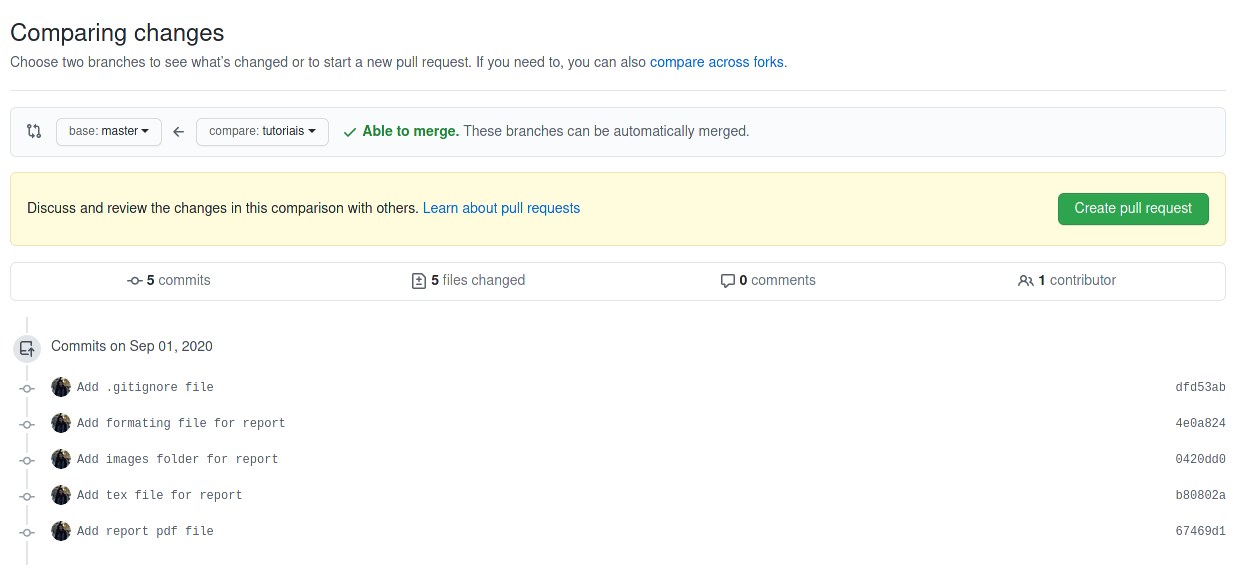
\includegraphics[width=15cm]{imagens/comparing_changes.png}
        \label{figura:comparing_changes}
    \end{figure}

    \begin{figure}[H]
        \caption{\textit{Antes de autorizar o \textit{merge}}}
        \vspace{0.5cm}
        \centering
        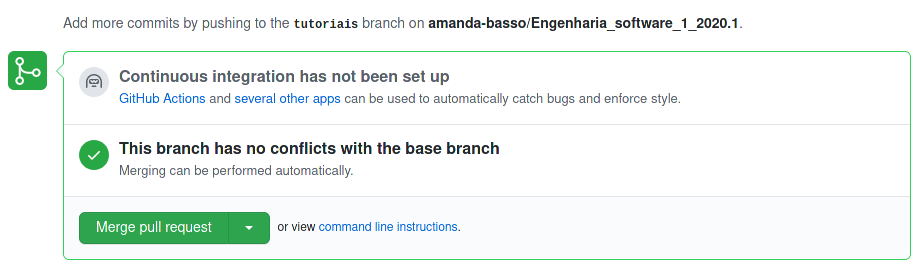
\includegraphics[width=15cm]{imagens/merge.png}
        \label{figura:merge}
    \end{figure}

    \begin{figure}[H]
        \caption{\textit{Pull request}}
        \vspace{0.5cm}
        \centering
        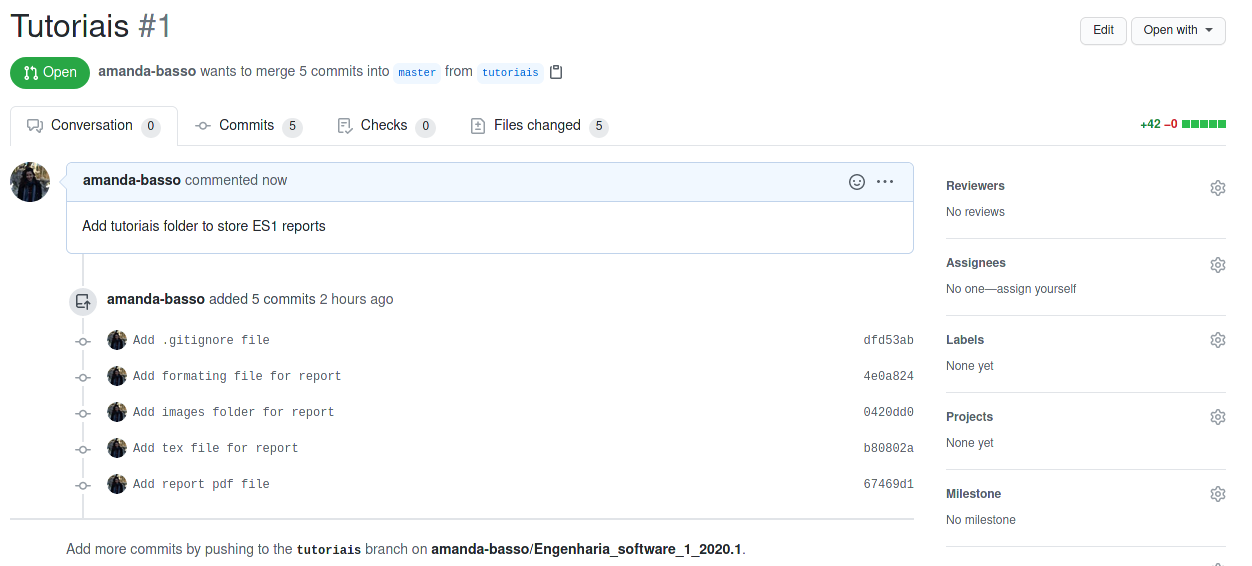
\includegraphics[width=15cm]{imagens/pull_request.png}
        \label{figura:pull_request}
    \end{figure}
